\documentclass[8pt]{beamer}
\usetheme{Goettingen}
\usecolortheme{dove}
\setbeamercovered{transparent}
\setbeamerfont{frametitle}{size=\normalsize} 
\setbeamertemplate{footline}[frame number]
\setbeamertemplate{itemize items}[circle]

\usepackage{mathrsfs} % equations
\usepackage{graphicx} % images
\usepackage[]{natbib} % citations + references
\bibliographystyle{unsrtnat} % citations + references


\title{Heat Kernel Smoothing}
\author[]{Gabriel Riegner}
\date{March 2025}

\begin{document}

% slide %
\begin{frame}{Heat Kernel Smoothing Using Laplace-Beltrami Eigenfunctions\\ \citep*{seo_heat_2010}}
\small
\begin{columns}
\column{0.5\textwidth}
\tableofcontents[hideallsubsections]
\column{0.5\textwidth}
\visible{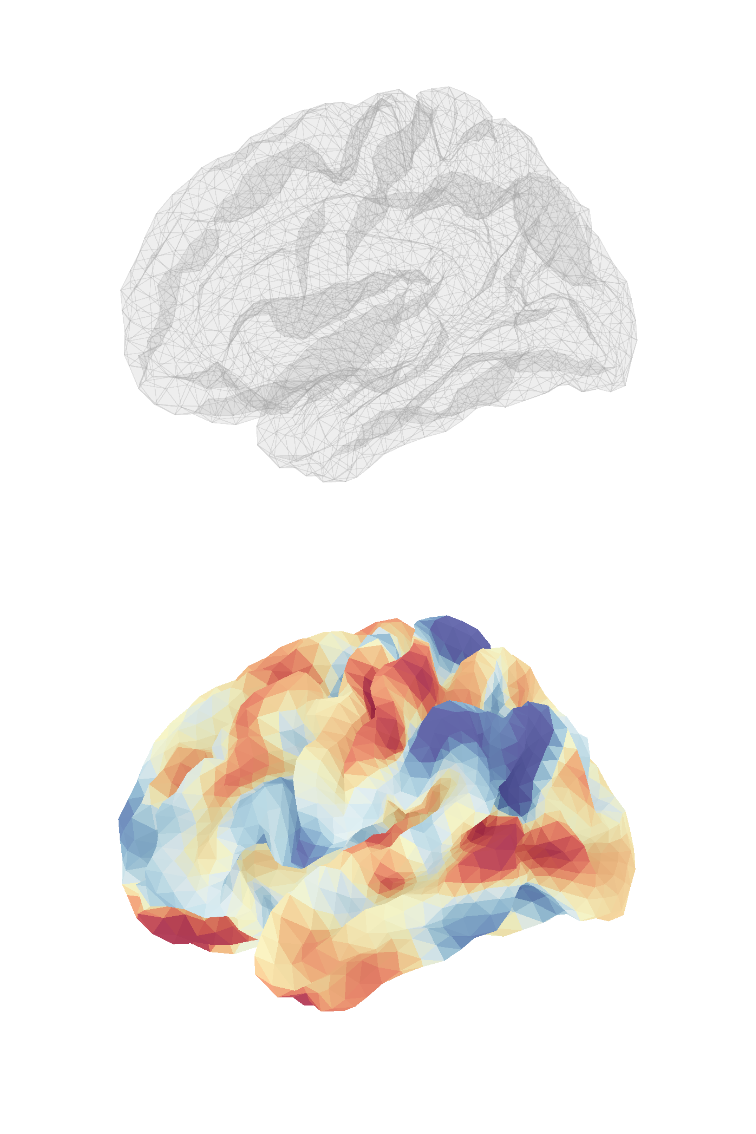
\includegraphics[width=0.8\textwidth]{project/figures/toc.png}}
\end{columns}
\vfill\centering
Gabriel Riegner, March 2025\\
DSC 291 Network Science and Graph Theory
\end{frame}


% section %
\section{Introduction}

\begin{frame}{Cortical Surface Data}
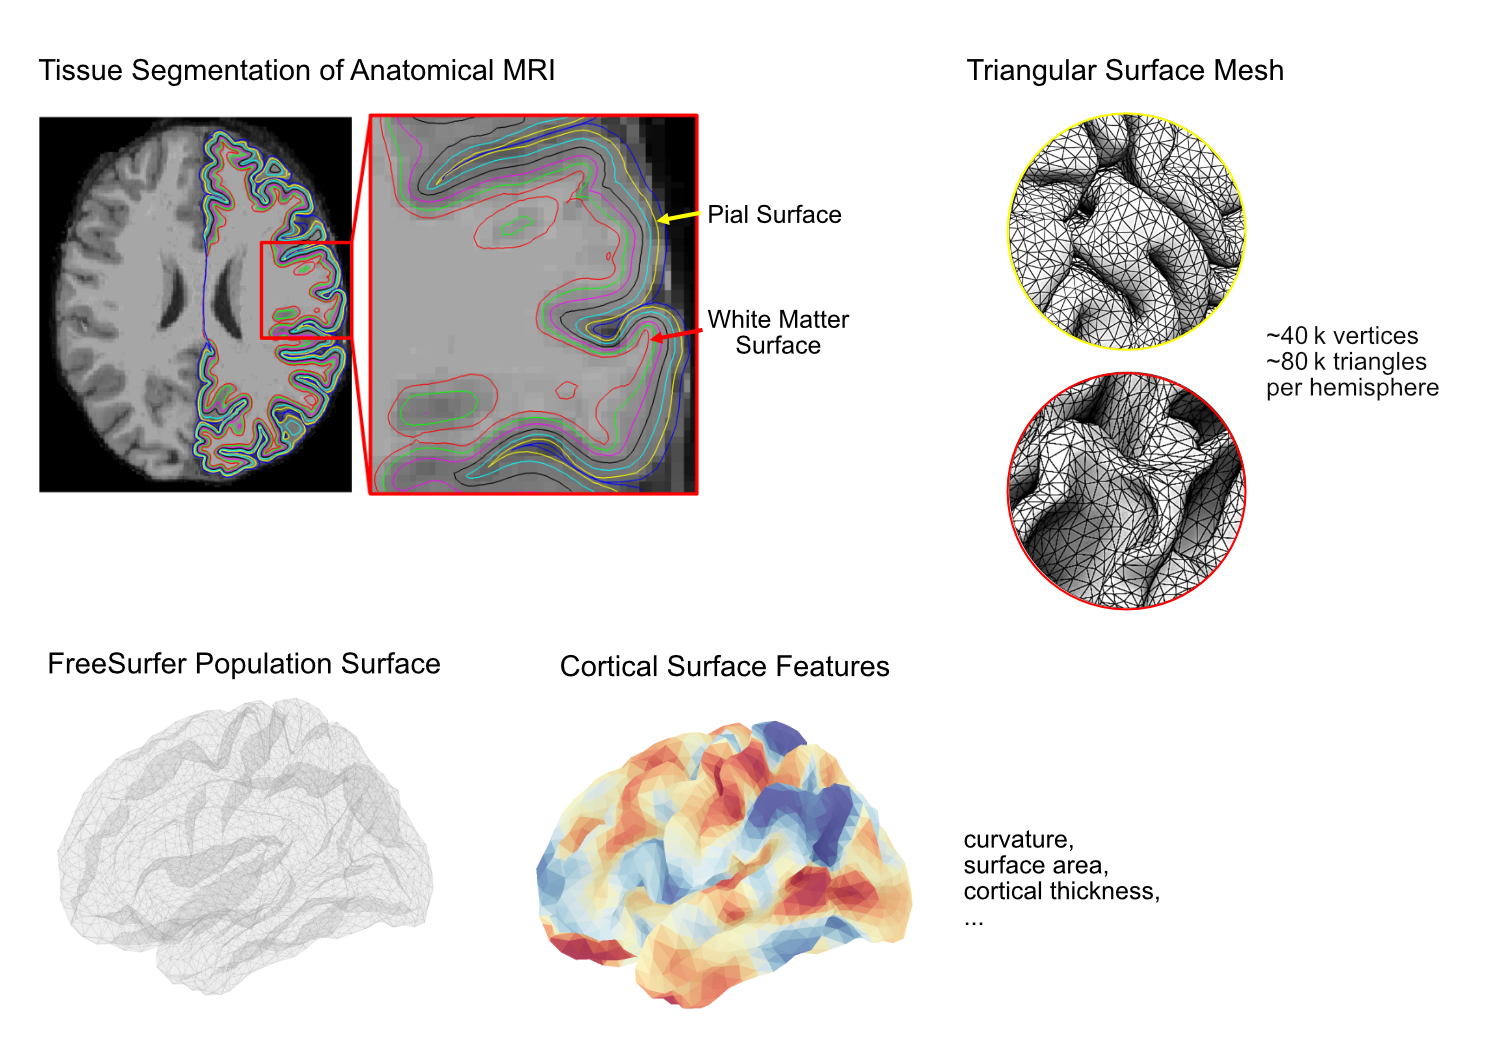
\includegraphics[width=1\textwidth]{project/figures/cortical-surface-data.png}    
\citep{dale_cortical_1999}
\end{frame}

\begin{frame}{Surface Distances}
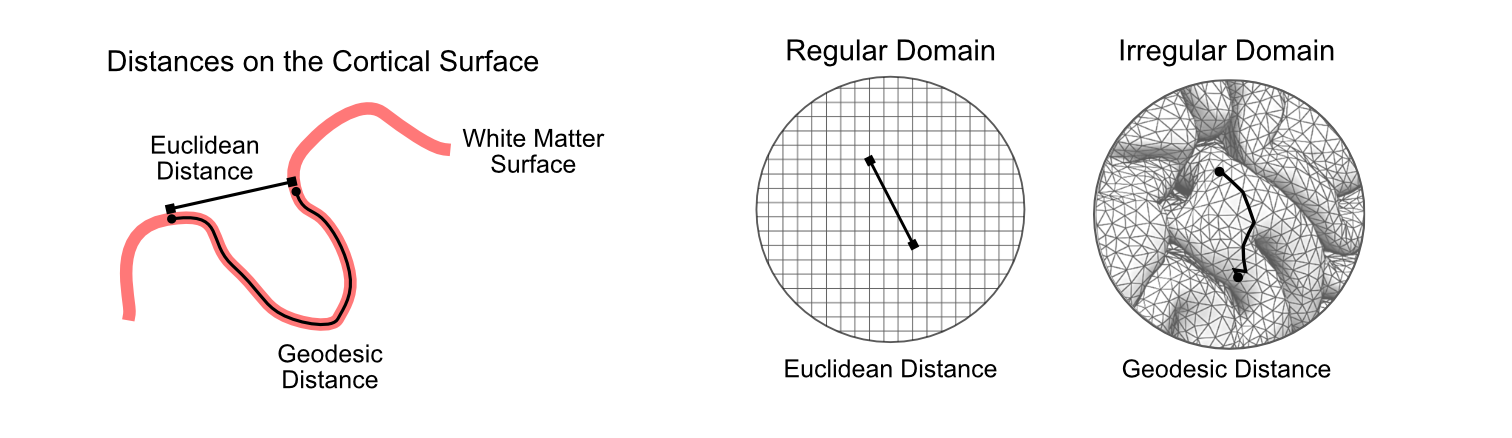
\includegraphics[width=1\textwidth]{project/figures/surface-distances.png} 
\end{frame}

% section %
\section{Paper Overview}

\begin{frame}{Surface Data Smoothing}
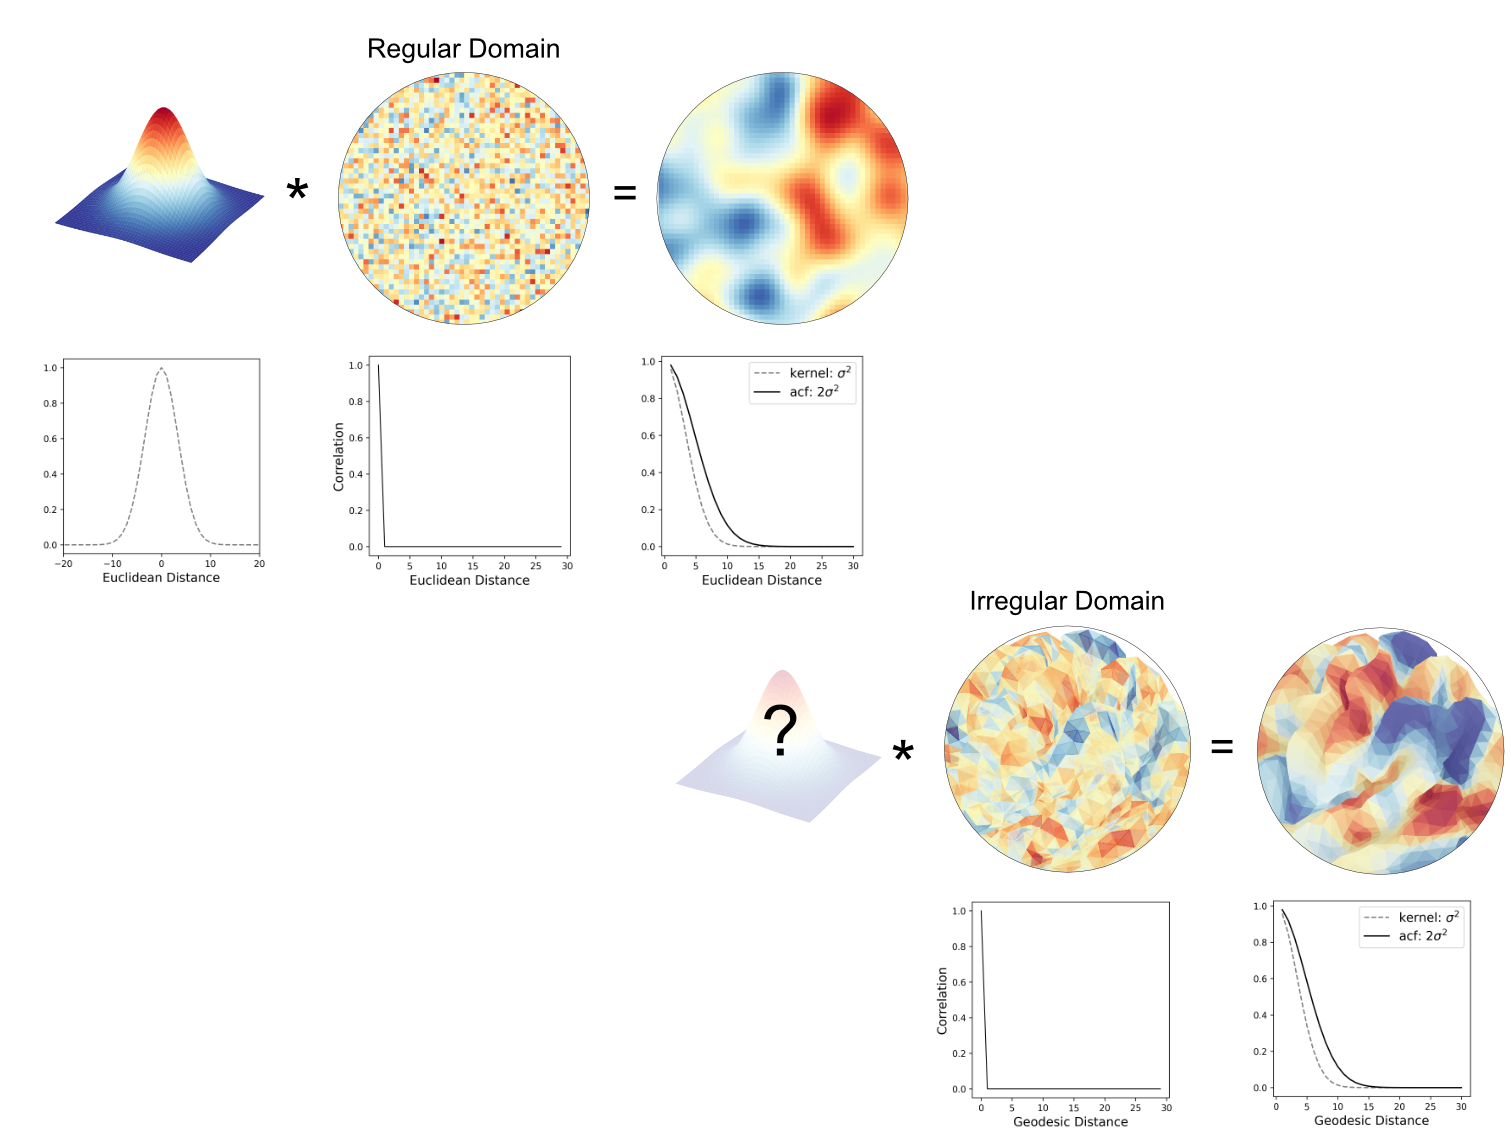
\includegraphics[width=1\textwidth]{project/figures/surface-data-smoothing.png}   
\citep{chung_discrete_2018, kushnarev_heat_2019}
\end{frame}

\begin{frame}{Definitions}
$Y$ defined on manifold $\mathcal{M} \subset \mathbb{R}^3$:
\begin{align}
    Y(p) = \theta(p) + \epsilon(p), \quad \epsilon(p) \overset{\text{iid}}{\sim} \mathcal{N}(0, \mathbb{I})
\end{align}

Eigenvalue problem for the Laplace-Beltrami operator $\Delta$ on $\mathcal{M}$:
\begin{align}
    \Delta \psi_j = -\lambda \psi_j
\end{align}

Heat kernel:
\begin{align}
    K_{\sigma}(p, q) = \sum_{j=0}^\infty e^{-\lambda_j\sigma} \psi_j(p) \psi_j(q)
\end{align}

Heat kernel smoothing:
\begin{align}
    Y_\sigma(p) \equiv K_{\sigma}  \ast Y(p) = \sum_{j=0}^\infty e^{-\lambda_j \sigma} \beta_j \psi_j(p)
\end{align}


Simplification:
\begin{align}
    z_j \equiv \beta_j = \langle Y, \psi_j \rangle \overset{iid}{\sim} \mathcal{N}(0, 1)
\end{align}

\citep{seo_heat_2010}
\end{frame}

\begin{frame}{Statistical Properties}
Mean:
\begin{align}
    \mathbb{E}[Y_\sigma(p)] = 0
\end{align}

Variance:
\begin{align}
    \mathbb{V}[Y_\sigma(p)] = \sum_{j=0}^\infty e^{-2\sigma\lambda_j}
\end{align}

Covariance:
\begin{align}
    \mathbb{C}[Y_\sigma(p), Y_\sigma(q)] = \sum_{j=0}^\infty e^{-\lambda_j 2\sigma} \psi_j(p) \psi_j(q)
\end{align}

Asymptotics:
\begin{align}
    \sigma&\to 0: Y_\sigma \to Y\\
    \sigma &\to \infty: Y_\sigma \to 0
\end{align}

\citep{kushnarev_heat_2019}
\end{frame}

% section %
\section{Contributions}

\begin{frame}{Graphs}
Laplace Matrix: $\Delta = D - A$
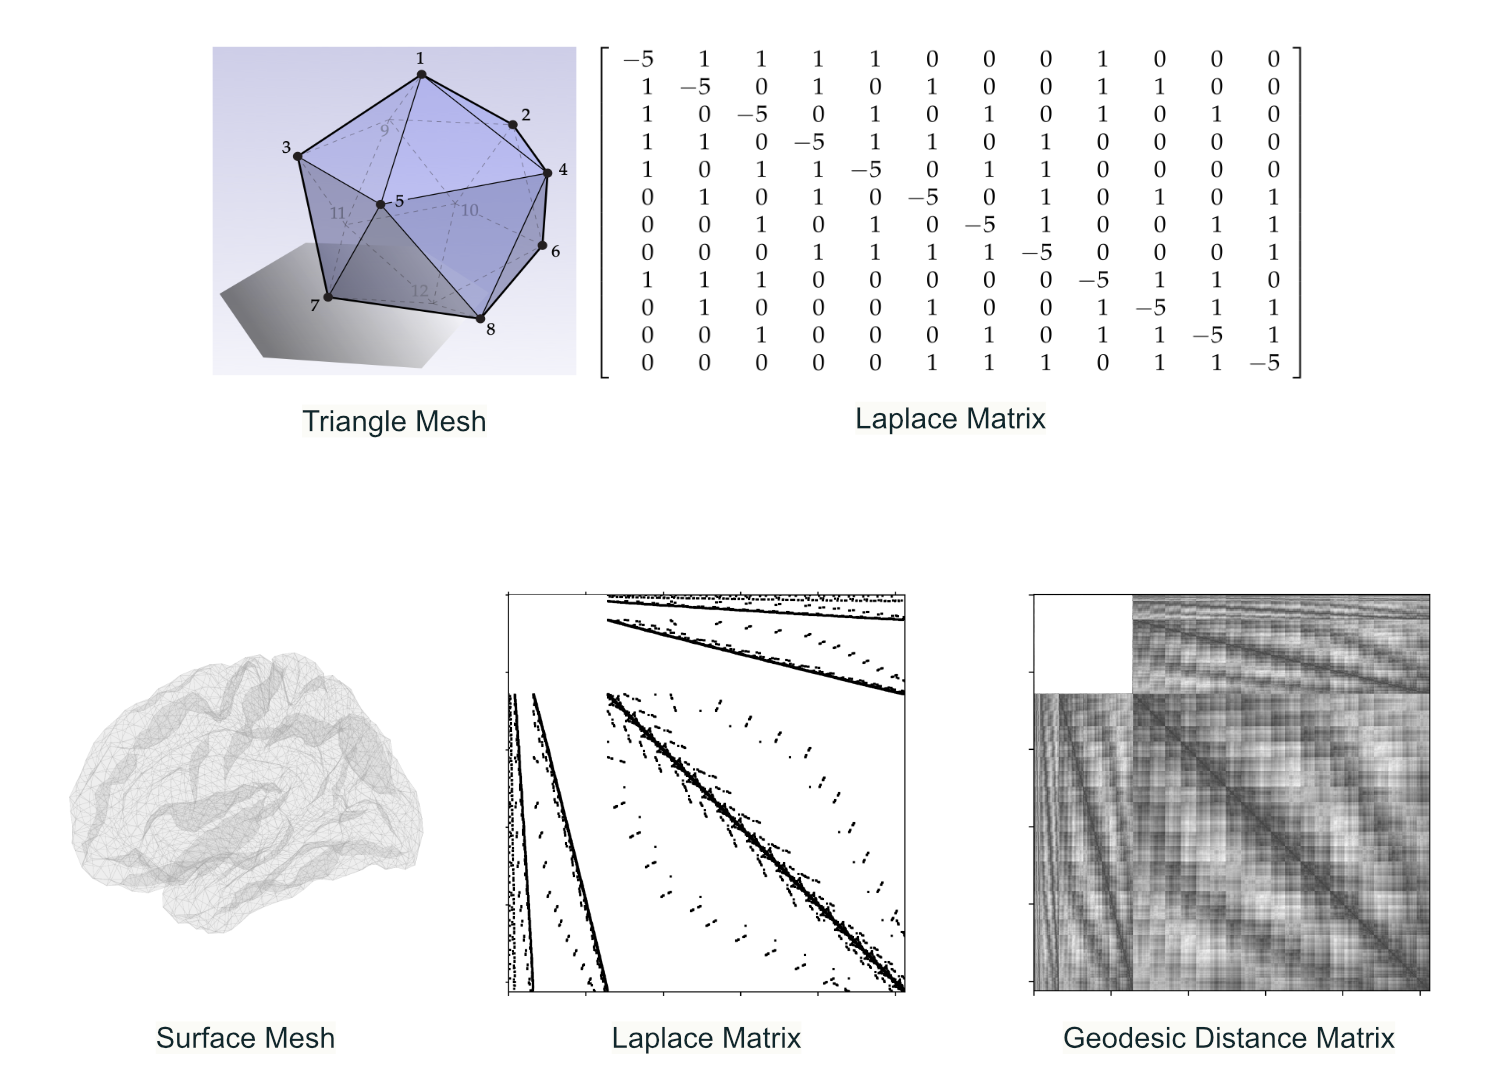
\includegraphics[width=1\textwidth]{project/figures/graphs.png}   
\citep{reuter_laplacebeltrami_2006}, [https://github.com/Deep-MI/LaPy]
\end{frame}

% section %
\section{Simulations}

\begin{frame}{Simulation Setting}
Eigenvalues:
\begin{align*}
    0 = \lambda_1 \le \lambda_2 \le \dots \le \lambda_k \tag{from 2}
\end{align*}

Eigenfunctions:
\begin{align*}
   \psi_1, \psi_2, \dots, \psi_k \tag{from 2}
\end{align*}

White noise:
\begin{align*}
    z_1, z_2, \dots, z_k \overset{iid}\sim \mathcal{N}(0, 1) \tag{from 5}
\end{align*}

\vspace{.25cm}
Heat Kernel Smoothing:
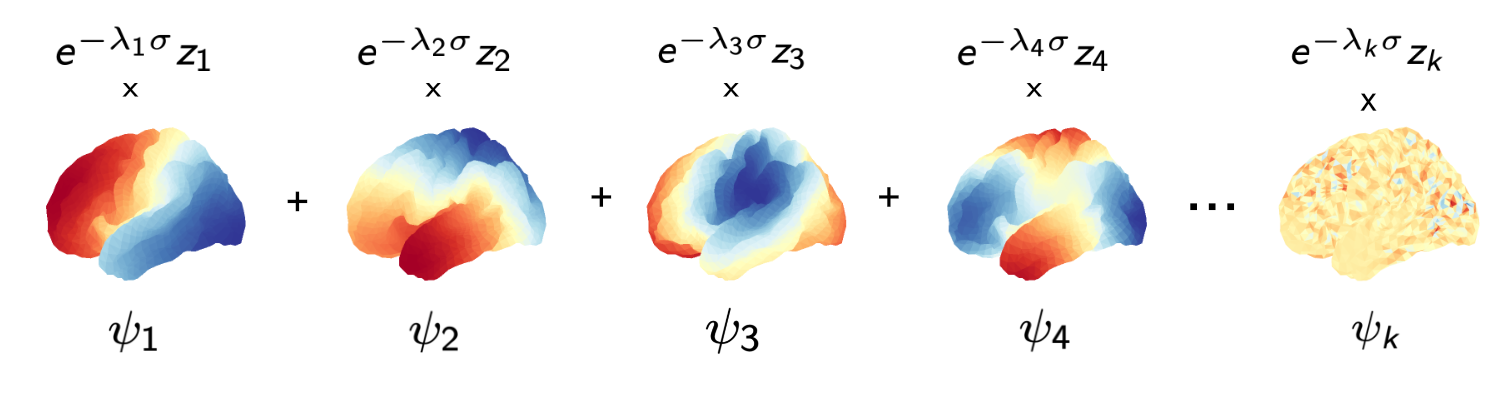
\includegraphics[width=1\textwidth]{project/figures/eigenfunctions.png}
\end{frame}

% section %
\section{Results}

\begin{frame}{Simulation Results}
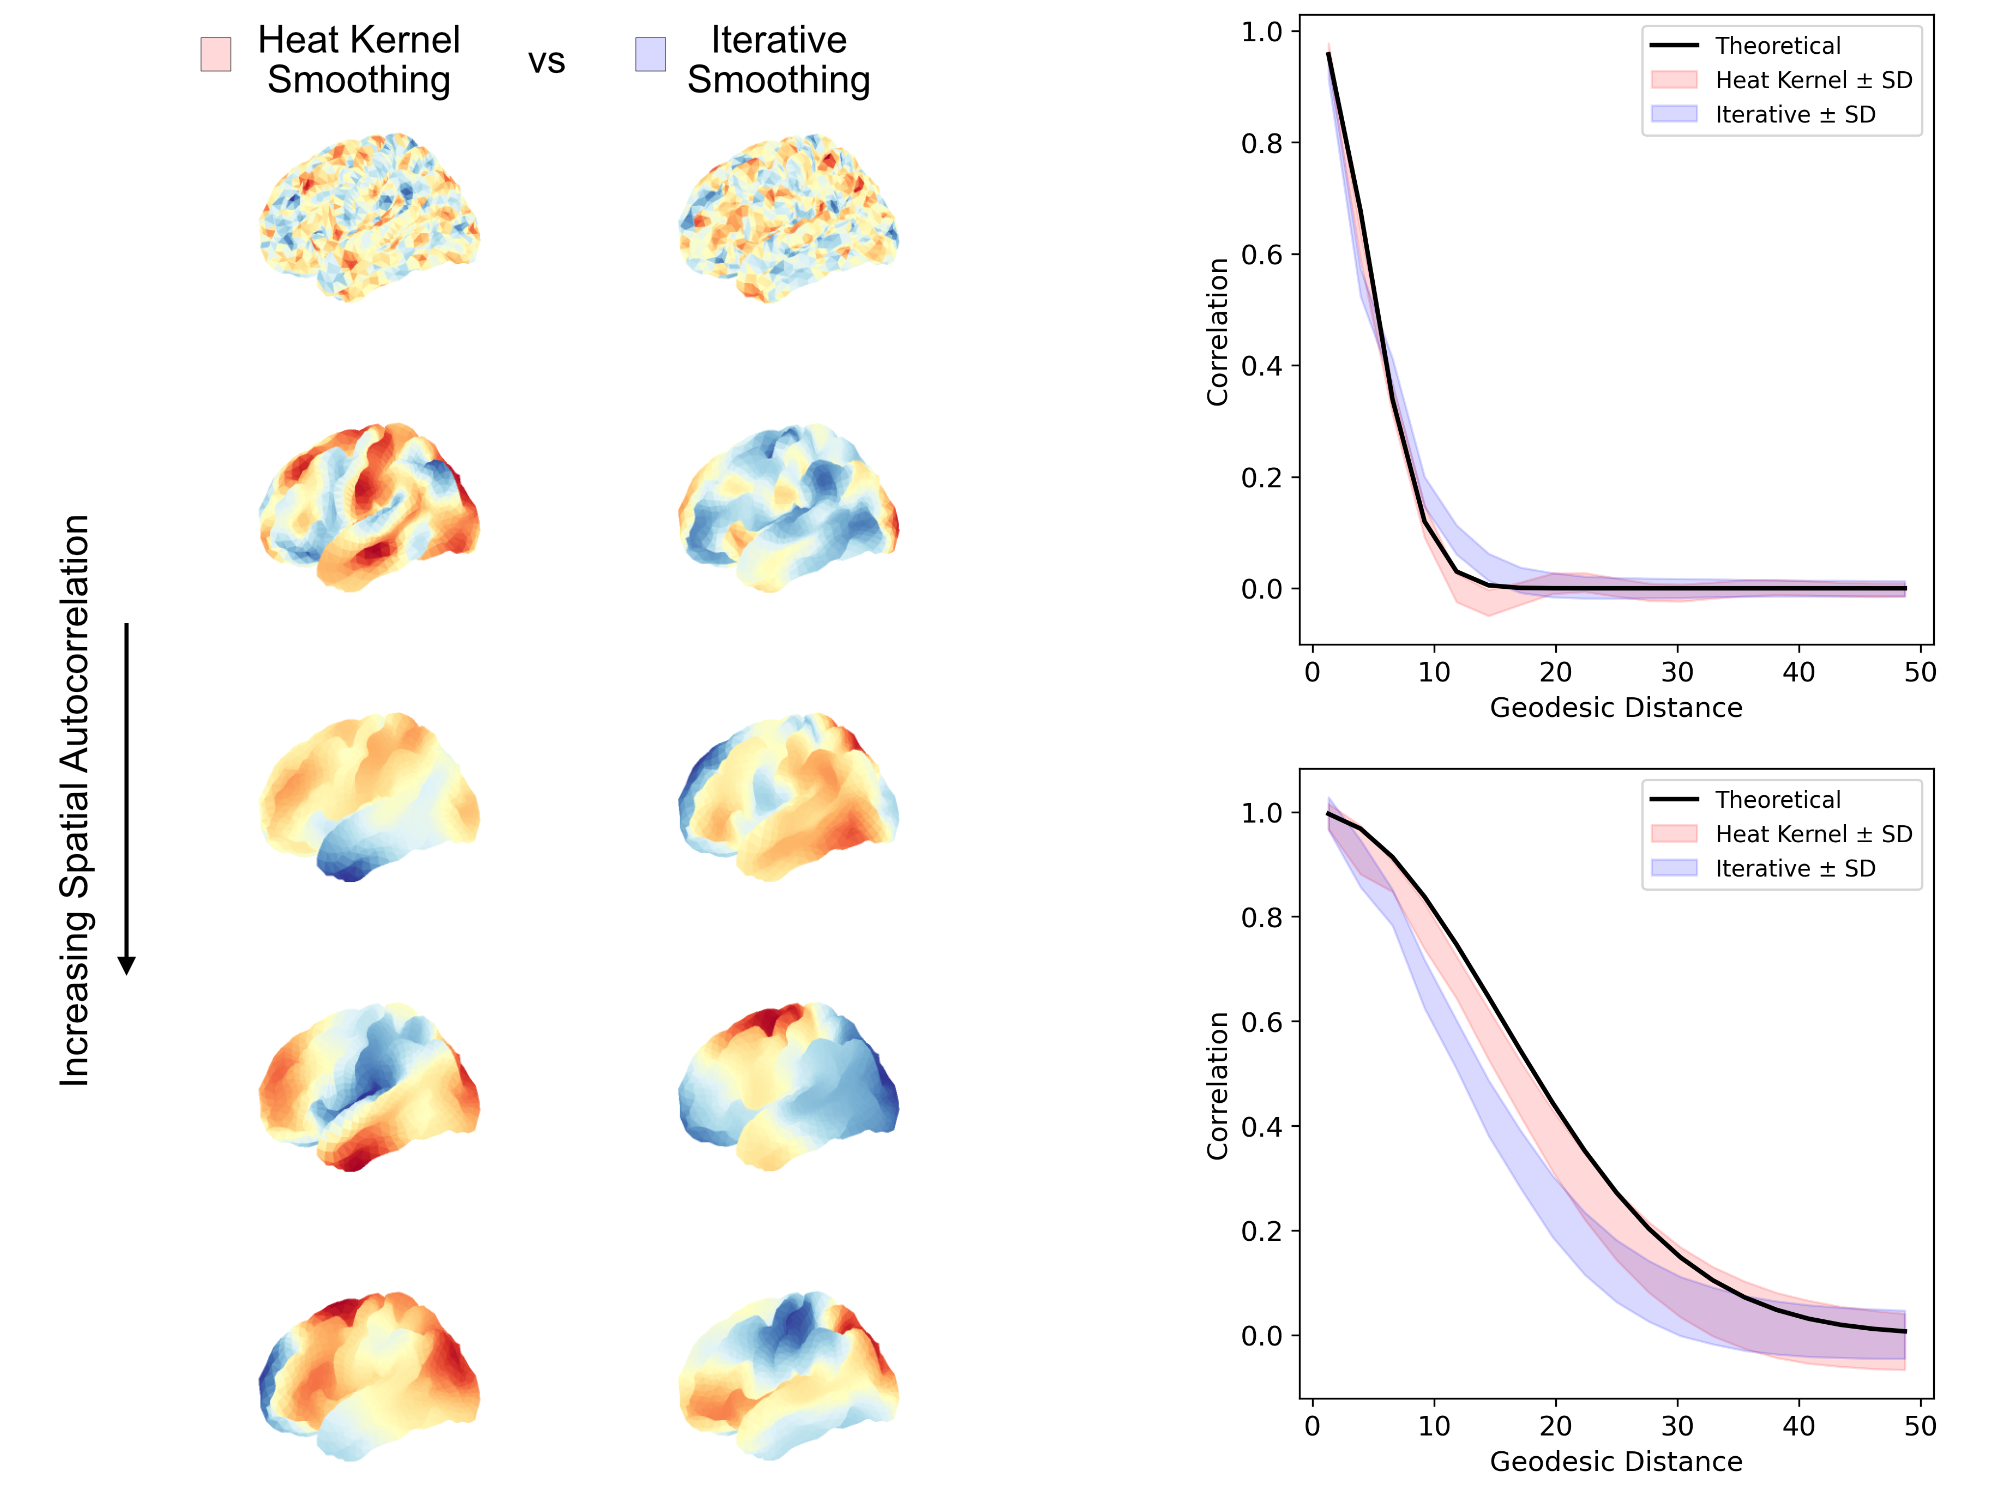
\includegraphics[width=1\textwidth]{project/figures/results.png}   
\end{frame}

% section %
\section{Conclusions}
\begin{frame}{Conclusions}
    \begin{itemize}
        \item \textbf{Geometry-aware smoothing}: Laplace-Beltrami eigenfunctions enable random field modeling on brain surfaces
        \vspace{0.5cm}
        \item \textbf{Spectral implementation}: Heat flow modeled via adjacency and Laplacian graphs
        \vspace{0.5cm}
        \item \textbf{Validated accuracy}: Simulations align with theoretical autocovariance decay with geodesic distance
        \vspace{0.5cm}
        \item \textbf{Computational efficiency}: Sparse Laplacian methods scale to large meshes (40k vertices)
    \end{itemize}
\end{frame}

% slide %
\begin{frame}{References}
    \small
    \bibliography{project/zotero}
\end{frame}

\end{document}